\documentclass[tikz, border=10pt]{standalone}
\usepackage{tikz}

\begin{document}
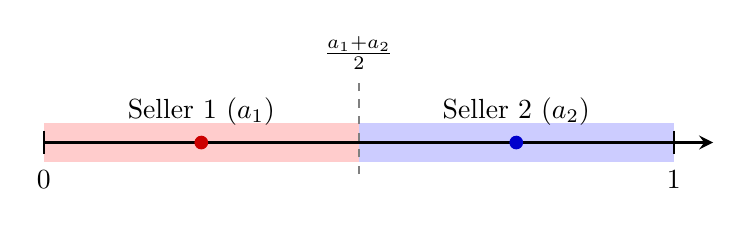
\begin{tikzpicture}[>=stealth]
  % Define coordinates (scaled manually to avoid distorting shapes)
  \def\xmin{0}
  \def\xmax{8}
  \def\sone{2}      % s_1 at 0.25
  \def\stwo{6}      % s_2 at 0.75
  \def\midpoint{4}  % Midpoint at 0.5

  % Color Regions (Occupied territory)
  \fill[red!20] (\xmin,-0.25) rectangle (\midpoint,0.25);
  \fill[blue!20] (\midpoint,-0.25) rectangle (\xmax,0.25);

  % Midpoint divider line
  \draw[dashed, thick, gray] (\midpoint,-0.4) -- (\midpoint,0.8);
  \node[above, black] at (\midpoint, 0.8) {$\frac{a_1 + a_2}{2}$};

  % Main Number Line
  \draw[very thick, ->] (\xmin,0) -- (\xmax + 0.5,0);

  % Endpoints
  \draw[thick] (\xmin, 0.15) -- (\xmin, -0.15) node[below=2pt] {$0$};
  \draw[thick] (\xmax, 0.15) -- (\xmax, -0.15) node[below=2pt] {$1$};

  % Store Locations (s1 and s2 as true circles)
  \node[circle, fill=red!80!black, inner sep=1.75pt, label={above:Seller 1 ($a_1$)}] at (\sone,0) {};
  \node[circle, fill=blue!80!black, inner sep=1.75pt, label={above:Seller 2 ($a_2$)}] at (\stwo,0) {};

  % Region Labels
  %\node[red!80!black, font=\bfseries] at (\midpoint/2, -0.6) {Seller 1 Market Share};
  %\node[blue!80!black, font=\bfseries] at (\midpoint + \midpoint/2, -0.6) {Seller 2 Market Share};

\end{tikzpicture}
\end{document}